\documentclass[20pt]{extarticle}

\usepackage{hyperref}
\usepackage{IEEEtrantools}
\usepackage{textcomp}
\usepackage{tikz}
\usepackage{pgfplots}
\pgfplotsset{compat=1.16}
\usepackage{adjustbox}
\usepackage{polynom}
\usepackage{amsmath}
% \usepackage{mathbb}

% inkscape figures
\usepackage{import}
\usepackage{xifthen}
\usepackage{pdfpages}
\usepackage{transparent}

\graphicspath{ {./figures/} }

% for inkscape-figures
\newcommand{\incfig}[1]{%
    \def\svgwidth{\columnwidth}
    \import{./figures/}{#1.pdf_tex}
}


% more space between IEEEeqnarray lines
\begin{document}{\setlength{\IEEEnormaljot}{15pt}
	% \section{A-level prep (holiday work)}
Work from \href{https://beechencliffmaths.weebly.com/as-prep-edexcel.html}{the weebly page}.
\subsection{Laws of indices}
When multiplying indices, add the exponents. When dividing indices, subtract them.
\begin{IEEEeqnarray}{rCl}
    x^m\times x^n & = & x^{m+n}
    \\
    \frac{x^m}{x^n} & = & x^{m-n}
\end{IEEEeqnarray}

For nested indices, multiply the exponents.
\begin{equation}
    (x^m)^n = x^{mn}
\end{equation}

Fractional indices take the form $\frac{\textrm{power}}{\textrm{root}}$.
\begin{equation}
    x^{\frac{m}{n}} = \sqrt[n]{x^m}
\end{equation}

Negative indices indicate ``one over''.
\begin{equation}
    x^{-m} = \frac{1}{x^m}
\end{equation}

Anything raised to the power 0 is 1.
\begin{equation}
    x^0 = 1
\end{equation}

\subsection{Surds}

\subsubsection{Key surd rules}

\paragraph{Multiplying}
\begin{equation}
    \sqrt{x} \sqrt{y} = \sqrt{xy}
\end{equation}

\paragraph{Dividing}
\begin{equation}
    \frac{\sqrt{x}}{\sqrt{y}} = \sqrt{\frac{x}{y}}
\end{equation}

\subsubsection{Simplifying surds}
To simplify a surd, find the largest square number that divides it.
\begin{IEEEeqnarray}{rCl}
    \sqrt{50} & = & \sqrt{25\times 2}\nonumber
    \\
    & = & 25\sqrt{2}
\end{IEEEeqnarray}

\subsubsection{Rationalising the denominator}
To rationalise the denominator of a fraction containing a surd, multiply by a fraction with that surd top and bottom (which is equal to 1).
\begin{IEEEeqnarray}{rCl}
    \frac{1}{\sqrt{3}} & = & \frac{1}{\sqrt{3}}\times \frac{\sqrt{3}}{\sqrt{3}} \nonumber
    \\
    & = & \frac{\surd{3}}{3}
\end{IEEEeqnarray}

For more complicated instances, the difference of two squares can be used.
\begin{IEEEeqnarray}{rCl}
    \frac{3}{2+\sqrt{5}} & = &
    \frac{3}{2+\sqrt{5}}\times \frac{2-\sqrt{5}}{2-\sqrt{5}}
    \nonumber \\
    & = & \frac{3(2-\sqrt{5})}{(2+\sqrt{5})(2-\sqrt{5})}
    \nonumber \\
    & = & \frac{6 - 3\sqrt{5}}{-1}
    \nonumber \\
    & = & 3\sqrt{5}-6
\end{IEEEeqnarray}

\subsection{Completing the Square}
Completing the square rearranges a quadratic from the form $ax^2+bx+c$ into the form $p(x+q)^2+r$. If $a \neq 1$, then this is done by factorising $a$ out of the first 2 terms.

\begin{IEEEeqnarray}{rCl?s}
    2x^2-5x+1 & = & 2\left(x^2+\frac{5}{2}x\right)+1 & // factorise out $a$
    \nonumber \\
    & = & 2\left[\left(x-\frac{5}{4}\right)^2-\left(\frac{5}{4}\right)^2\right]+1 & // CTS inner part
    \nonumber \\
    & = & 2\left(x-\frac{5}{4}\right)^2-\frac{25}{8}+1 & // multiply out
    \nonumber \\
    & = & 2\left(x-\frac{5}{4}\right)^2-\frac{7}{8}+1 & // simplify
\end{IEEEeqnarray}
	% %! TEX root = /home/tc/school/alevel/Maths/master.tex
\section{Representations of quadratics}
Consider the quadratic equation $ax^2+bx+c=0$ (and/or its graph, $y=ax^2+bx+c$). Given the quadratic in this form, and assuming that $a=1$ and also that the quadratic will factorise (these things are assumed throughout this section), we can find other useful information about (or if you want to think about it this way, forms of) this quadratic.

\subsection{Y-intercept}
The point at which the quadratic's graph crosses the y-axis, or rather, its coordinate when $x=0$. It is $c$ from $y=ax^2+bx+c$, because when $x=0$, $ax^2+bx$ must also equal $0$.
\begin{IEEEeqnarray}{sL}
    Equation: & y=x^2+2x-24
    \nonumber \\
    Y-intercept: & (0, -24)
\end{IEEEeqnarray}

\subsection{Factorisation}
A factorised version of the quadratic in the form $(x+m)(x+n)$. Useful for finding the roots. For $y=ax^2+bx+c$, $m$ and $n$ are two numbers that sum to $a$ and multiply to $b$.
\begin{IEEEeqnarray}{sL}
    Equation: & y=x^2+2x-24
    \nonumber \\
    Factorisation: & (x+6)(x-4)
\end{IEEEeqnarray}

\subsection{Roots}
The roots (or solutions) are the values of $x$ that satisfy $ax^2+bx+c=0$. They are also the x-coordinates at which $y=ax^2+bx+c$ crosses the x-axis. To find them, take $m$ and $n$ from the quadratic's factorisation, and multiply by $-1$.
\begin{IEEEeqnarray}{sL}
    Factorisation: & (x+6)(x-4)
    \nonumber \\
    Roots: & x=-6 \textrm{ or } x=4
\end{IEEEeqnarray}

\subsection{Completed the square}
This version takes the from $(x+p)^2+q$. It's useful for finding the turning points of the graph. For $y=ax^2+bx+c$, $p=\frac{b}{2}$, and $q=c-q^2$.
\begin{IEEEeqnarray}{sL}
    Equation: & y=x^2+2x-24
    \nonumber \\
    Completed the square: & (x+1)^2-25
\end{IEEEeqnarray}

\subsection{Turning point}
The turning point of the graph, found using the completed the square form of the equation. The x-coordinate is $-p$, because this would make the entire expression as small as possible ($0$, because no square term can be smaller), and the y-coordinate is simply $q$, because that will be all that's left when $(x+p)^2=0$.
\begin{IEEEeqnarray}{sL}
    Completed the square: & (x+1)^2-25
    \nonumber \\
    Turning point: & (-1, -25)
\end{IEEEeqnarray}

\subsection{Sketch}
Sketches of the graph should have their intercepts labelled, as well as the turning point.

So for $y=x^2+4x+3$ (the other one was too big to draw nicely):

\adjustbox{margin=1cm}{
    \pgfplotsset{ticks=none}
    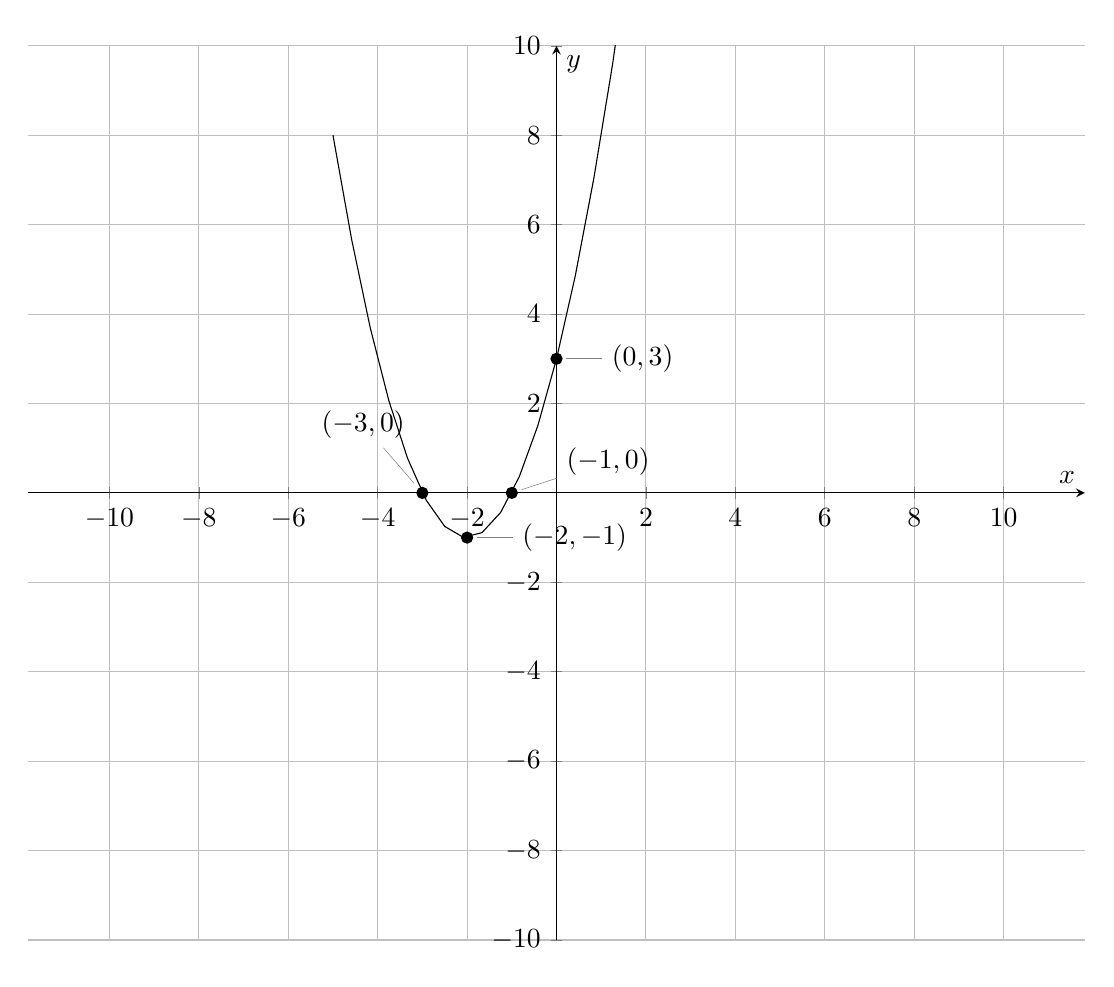
\begin{tikzpicture}[baseline]
        \begin{axis}[
            axis y line=center,
            axis x line=middle,
            axis equal,
            grid=both,
            xmax=10,xmin=-10,
            ymin=-10,ymax=10,
            xlabel=$x$,ylabel=$y$,
            width=15cm,
            anchor=center,
            ]
            \addplot[mark=none] {x^2+4*x+3};
            \addplot[mark=*] coordinates {(-2,-1)} node[pin=right:{$(-2, -1)$}]{} ;
            \addplot[mark=*] coordinates {(-3,0)} node[pin=100:{$(-3, 0)$}]{} ;
            \addplot[mark=*] coordinates {(-1,0)} node[pin=10:{$(-1, 0)$}]{} ;
            \addplot[mark=*] coordinates {(0,3)} node[pin=right:{$(0, 3)$}]{} ;
        \end{axis}
    \end{tikzpicture}
}

\section{Properties of quadratics}
There are certain key properties of quadratics in the form $ax^2+bx+c$.

\subsection{Factorising with integers}
This means that the quadratic can be factorised into the form $(ax+b)(cx+d)$ where $a$, $b$, $c$, and $d$ are all integers. Only some quadratics have this property. You can find out whether a quadratic has an integer factorisation by putting it into the quadratic formula $\frac{-b\pm\sqrt{b^2-4ac}}{2a}$. If the discriminant (the part under the square root) is a square number, then the quadratic can be factorised with integers, otherwise it cannot.

\subsection{Two x-intercepts}
This means that the quadratic's graph crosses the x-axis at 2 points, and therefore means that there are 2 different solutions to the equation when the quadratic is set equal to 0.

\subsection{Repeated x-intercept}
This means that the quadratic's graph touches the x-axis at only one point. If the quadratic factorised, it would be in the form $(ax+b)^2$. Setting the quadratic equal to 0 would only yield one solution.

\subsection{No x-intercepts}
This means that the quadratic's graph stays above or below the x-axis at all times, never touching it at any point. Any quadratics that have this property definitely will not factorise with integers, as this would imply it having either one or two x-intercepts. In fact, when set equal to 0, these quadratics have no real solutions.

\subsection{Has a minimum point}
This means that the quadratic's graph is `happy' (looks like a smiley face, with the turning point as the lowest point in the graph, and the graph extending infinitely upwards). Quadratics in the form $ax^2+bx+c$ where $a>0$ have this property.

\subsection{Has a maximum point}
This means that the quadratic's graph is `unhappy' (looks like an upside-down smiley face, with the turning point as the highest point in the graph, and the graph extending infinitely downwards). Quadratics in the form $ax^2+bx+c$ where $a<0$ have this property.

\subsection{Y-intercept}
The point at which the quadratic's graph crosses the y-axis. Equal to $c$ for quadratics in the form $ax^2+bx+c$.

\section{Quadratics in disguise}
Some quadratics may be disguised. For example, if there are other indices involved before the term gets squared. For example:
\begin{IEEEeqnarray}{rCl?s}
    x^4 + x^2 + 4 & = & 0 & // can be rewritten as
    \nonumber \\
    (x^2)^2 + (x^2) + 4 & = & 0 & // let $y = x^2$
    \nonumber \\
    y^2 + y + 4 & = & 0 & // and solve normally
\end{IEEEeqnarray}
Don't forget, after solving for $y$, to then sub $x^2$ back in and solve for $x$

This can also happen with fractions ($x^{\frac{2}{3}}+x^{\frac{1}{3}}+3$), or addition when $x$ is used in the exponent ($4^{2x}+4^{x+1}+6$). In each case, find something to substitute so that you're left with a term squared, followed by that same linear term, followed by constant. Then it should be fine to solve, for the substituted variable, substitute $x$ back in, and solve for $x$.

\section{The Discriminant}
In the quadratic formula $x=\frac{-b\pm \sqrt{b^2-4ac}}{2a}$, the part under the square root symbol, ($b^2-4ac$), is called the discriminant. It is useful for finding certain properties of quadratics:
\begin{itemize}
    \item If $b^2-4ac > 0$: the quadratic has 2 real roots.
    \item If $b^2-4ac = 0$: the quadratic has 1 repeated root.
    \item If $b^2-4ac < 0$: the quadratic has no real roots.
    \item If $b^2-4ac$ is a square number, then the quadratic factorises with integers.
\end{itemize}

\section{Quadratic inequalities}
Quadratic inequalities can be thought of as finding part of a graph. For example, solving the inequality $x^2-2<0$, can be thought of as finding all of the x-values for which the graph $y=x^2-2$ goes below the $x$-axis. As such, the correct way to solve a quadratic inequality is to get everything onto one side of the inequality sign, and then you can find the roots (called \b{critical values} for inequalities), and work out which part of the graph you're after.

\section{Quadratic simultaneous equations}
Quadratic simultaneous equations can be solved with substitution, similar to normal inequalities. However, they can also once again be thought of in terms of the relevant graphs. For example, solving the simultaneous equations:
\begin{IEEEeqnarray}{rCl}
    x^2 + y^2 & = & 25
    \nonumber\\
    y & = & 2x + 4
\end{IEEEeqnarray}
can be thought of as finding where their graphs intersect:
\adjustbox{margin=1cm}{
    \pgfplotsset{}
    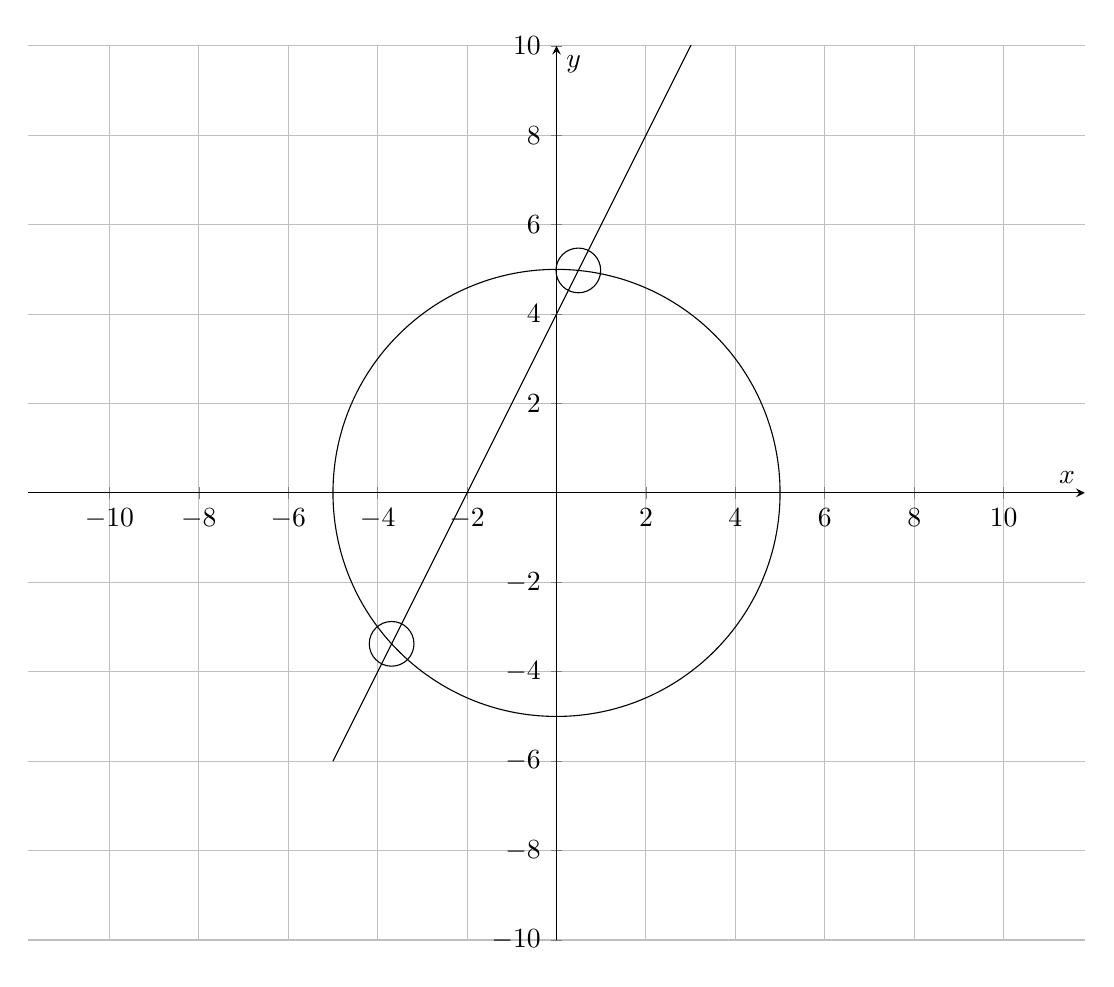
\begin{tikzpicture}[baseline]
        \begin{axis}[
            axis y line=center,
            axis x line=middle,
            axis equal,
            grid=both,
            xmax=10,xmin=-10,
            ymin=-10,ymax=10,
            xlabel=$x$,ylabel=$y$,
            width=15cm,
            anchor=center,
            ]
            \draw (axis cs:0,0) circle [black, radius=5];
            \draw (axis cs:0.488,4.976) circle [blue, radius=0.5];
            \draw (axis cs:-3.688,-3.376) circle [blue, radius=0.5];
            \addplot[mark=none] {2*x+4};
        \end{axis}
    \end{tikzpicture}
}

	% \section{Algebra tricks}
Various useful algebraic tricks that can be tried when stuck on a problem.
\subsection{Forcing the denominator into the numerator}
\begin{IEEEeqnarray}{Cl}
    & \frac{x^2}{x^2-9}
    \nonumber \\
    \equiv & \frac{(x^2+9)+9}{x^2-9}
    \nonumber \\
    \equiv & \frac{x^2-9}{x^2-9}+\frac{9}{x^-9}
    \nonumber \\
    \equiv & 1+\frac{9}{x^-9}
\end{IEEEeqnarray}
	% \section{Line Graphs}
\subsection{Working out a line between two points}
First use $m=\frac{\Delta y}{\Delta x}$, substituting in the coordinates of the two points to find $m$. Then, substitute this value of $m$, as well as the coordinates from one of the points, into $y=mx+c$. You can solve to find c, and then you have your line equation.
\subsection{Are they parallel?}
If they have the same gradient, then yes.
\subsection{Are they perpendicular?}
If their gradients multiply to -1, then yes.

\section{Lengths and Areas}
To find the distance between two points on a cartesian grid, we can create a right angled triangle and thereby use pythagoras to find the distance. That is to say, for the coordinates $A (x, y)$, and $B (x_1, y_1)$, then the distance between them is equal to $\sqrt{(x-x_1)^2+(y-y_1)^2}$.

\adjustbox{margin=1cm}{
    \pgfplotsset{}
    \begin{tikzpicture}[baseline]
        \begin{axis}[
            axis y line=center,
            axis x line=middle,
            axis equal,
            grid=both,
            xmax=5,xmin=-5,
            ymin=-5,ymax=5,
            xlabel=$x$,ylabel=$y$,
            width=10cm,
            anchor=center,
            ]
            \addplot coordinates {(1,4) (5,4)};
            \addplot coordinates {(1,4) (1,0)};
            \addplot coordinates {(1,0) (5,4)};
        \end{axis}
    \end{tikzpicture}
}

\section{Linear models}
Linear models can be used to represent the relationships between variables. For example, between a the mass on a spring and its extension, or between the amount of a product / duration of a service and its price.

\subsection{Is a linear model suitable?}
To find out whether a linear model is suitable for some given data, plot the data on the graph and see if the points fall roughly  on a straight line. If they do, an equation can be worked out by using the two given data points that are furthest away for the gradient.

\subsection{Explaining variables in linear models}
Questions will often require explaining what the gradient and the y-intercept refer to. The gradient can be described as the how much one variable changes \b{per} unit of change in the other. The y-intercept differs between questions. Examples might be the level of one variable when we started measuring, the flat fee charged for the service/product, or something else entirely. This just requires common sense.

	% \section{Circles}
\subsection{Equations of circles}
\subsubsection{Circles with centres at the origin}
For any circle with centre $(0, 0)$ and radius $r$, the equation of the circle is $x^2+y^2=r^2$.
\subsubsection{Circles not centered at the origin}
If the circles are not centered at the origin, the rules for transforming graphs apply. This means that for a circle centre $(a, b)$, radius $r$, the equation would be $(x-a)^2+(x-b)^2=r^2$

\subsection{Common types of question}
\subsubsection{Finding centre and radius}
This is a common type of question. You could be given for example the centre and a point the circle passes through, or perhaps the equation in its expanded form. The first of these isn't too difficult, as the radius can be found using Pythagoras' theorem. For the latter, the best thing to do is to complete the square on the $x$ annd $y$ terms separately, before moving everything else to the other side of the equation. For example:
\begin{IEEEeqnarray}{rCls}
	x^2+y^2-14x+16y-12 & = & 0
	\nonumber\\
	x^2-14x+y^2+16y-12 & = & 0 & // Group related terms
	\nonumber\\
	(x+7)^2-49+(y+8)^2-64-12 & = & 0 & // Complete the square
	\nonumber\\
	(x+7)^2(y+8)^2 & = & 125 & // Move linear terms to RHS
\end{IEEEeqnarray}

\subsection{Intersections with straight lines}
If a line touches a circle, then you can solve them as simultaneous equations to work out where they intersect. If a line is a tangent to the circle, the simultaneous equations will only have one solution, and if they don't intersect at all, there won't be any solutions.
\subsubsection{A common lines and circles exam question}
Often, you'll be given equation of a circle, and the y-intercept of a line tangent to that circle. In this case, you can find the equation of the line by substituting in that $y=mc+c$ (you know $c$), and forming a quadratic. Next, because you know that the line is a tangent, you know that the quadratic must have one solution, and you can use the discriminant to create another quadratic in terms of $m$ and solve it before reconstructing the equation of the line.

\subsection{Circumcircles}
A circumcircle is a circle that touches all three corners of a triangle. These can be drawn for any triangle by constructing perpendicular bisectors between two of the three edges. The point at which they meet is the centre of this circle (called a \textbf{circumcentre}).
\subsection{Proving that one of the lines is a diameter}
For a right-angled triangle, then the hypotenuse will be the diameter of its circumcircle. You can use the circle theorem that the angle at the circumference of a semicircle is 90\textdegree{} to prove this.

	% \section{Polynomials}
A polynomial is a finite expression with positive whole number indices.
\subsection{Long division of polynomials}
This can be used to see what the remainder is when a polynomial is divided by $(x+p)$ where $p$ is a constant term. For example, to divide $x^3+2x^2-17x+6$ by $x+3$, you could set it out something like this:

\polylongdiv{x^3+2x^2-17x+6}{x+3}

The part left at the top is called the \textbf{quotient}, while the linear term left at the end is the \textbf{remainder}. This is really telling us that $x^3+2x^2-17x+6=(x+3)(x^2-x-14)+48$.

\subsubsection{Missing terms in long division}
If a term is missing, it needs to be replaced with a $+0$ times the missing term so that the method still works.

\subsection{The factor theorem}
The factor theorem states that for any polynomial $f(x)$, the statement ``$(x-a)$ is a factor of $f(x)$'' is equivalent to saying that ``$f(a)=0$''. This means that you can use the factor theorem to prove that something is a factor of a polynomial by substituting in $a$ in $(x-a)$ and showing that the output is equal to $0$.


	% \section{Proof}
A proof is a demonstration that a mathematical statement is true, which only uses already known facts.

\subsection{Theorems vs conjectures}
This is a simple difference. A theorem is a statement that has been proved to be correct, while a conjecture is a statement that is yet to be proved.

\subsection{Types of proof}
\subsubsection{Proof by deduction}
This is the simplest kind of proof. It may often involve algebra, and will directly show the statement is true.
\subsubsection{Proof by exhaustion}
This works by proving every single possible case. As such, it is not always useable for all statements.
\subsubsection{Proof by contradiction}
This kind of proof works by assuming that the negation of a statement is true, and then doing something with the negation that leads to a false statement, thus proving the original non-negated version of the statement in question.
\subsubsection{Disproof by counterexample}
Fairly self-explanatory
\subsubsection{Proof by induction}
Don't need to know until later on in the course. Works by proving the statement for one case, and then proving that if it works for case $k$ it must also work for case $k+1$.

\subsection{Setting out proofs}
When setting out proofs, it is important to start with the true statement and work towards the statement in question. It's ok to have jottings that do this in the reverse order, but the proof must then be formally written out with the correct order of statements as well to gain the marks.

	% \section{Graphs}
\subsection{Sketching cubic graphs}
When sketching a cubic graph, you need it in its factorised form. Then, you can find the y-intercept by multiplying all of the linear parts of each factorised term together, and find the x-intercepts in the same way in which you would for a quadratic. If a root is repeated, then the graph will just touch the $x$-axis at that point. Cubics will always follow the same general shape depending on whether they have a positive or negative coefficient of $x^3$. Examples could be:

\begin{figure}[ht]
    \centering
    \incfig{examples-of-cubic-graphs}
    \caption{Examples of cubic graphs. Left with positive $x^3$ coefficients, right with negative ones.}
    \label{fig:examples-of-cubic-graphs}
\end{figure}

\subsection{Quartic graphs}
Quartic graphs can have many different shapes (examples below). Sketching them is similar to sketching cubics.

\begin{figure}[ht]
    \centering
    \incfig{examples-of-quartic-graphs}
    \caption{Examples of quartic graphs. Bottom right with a negative $x^4$ coefficient.}
    \label{fig:examples-of-quartic-graphs}
\end{figure}

\subsection{Reciprocal graphs}
Reciprocal graphs are characterised by having \textbf{asymptotes}, which are lines which the graph gets infinitely close to without touching it. We can sketch these graphs by considering what will happen in each quadrant (often by trying the function with different inputs or outputs), and considering these asymptotes.

\begin{figure}[ht]
    \centering
    \incfig{examples-of-reciprocal-graphs}
    \caption{Examples of reciprocal graphs}
    \label{fig:examples-of-reciprocal-graphs}
\end{figure}

\subsubsection{Comparing reciprocal graphs}
Some questions might ask for multiple reciprocal graphs to be drawn on the same axes. For this scenario, it's best to think which graph will be higher at any given point. For example, $y=\frac{1}{x}$ will always be lower down than $y=\frac{2}{x}$ with the same $x$-value.

\subsection{Points of intersection of graphs}
The points at which $y=f(x)$ and $y=g(x)$ intersect are the solutions to the equation $f(x)=g(x)$. This means that we can solve the equation by sketching the graphs, as well as finding the points of intersection by solving the equation. Another possible question might be to say how many solutions an equation has without using the discriminant or some other method. In this case, sketching both sides of the equation is enough to deduce the answer.

\subsection{Transformations of graphs}
By manipulating graphs' equations in different ways, we can transform them in different ways on a grid.
\subsubsection{Translations}
$f(x)$ moves $a$ units up when it becomes $f(x)+a$. This is a translation by the vector $\begin{pmatrix}0 \\ a\end{pmatrix}$.

$f(x)$ moves $a$ units to the left when it becomes $f(x+a)$. This is a translation by the vector $\begin{pmatrix}-a \\ 0\end{pmatrix}$.

\subsubsection{Stretches}
When $f(x)$ becomes $af(x)$, it is stretched in the $y$ direction with a scale factor of $a$.

When $f(x)$ becomes $f(xa)$, it is stretched in the $x$ direction with a scale factor of $\frac{1}{a}$.

\subsubsection{Reflections}
Reflections are just special cases of stretches where the scale factor is $-1$. So, a reflection in the x-axis would be $f(x)$ becoming $-f(x)$, while a reflection in the y-axis would be $f(x)$ becoming $f(-x)$.

	% \section{Trigonometry}
\begin{figure}[ht]
    \centering
    \incfig{a-triangle-labelled-for-the-sin-and-cosine-rules}
    \caption{A triangle labelled for the sin and cosine rules}
    \label{fig:a-triangle-labelled-for-the-sin-and-cosine-rules}
\end{figure}
\subsection{The cosine rule}
The cosine rule states that for any triangle with the angles labelled as $A$, $B$, and $C$, and the sides opposite them labelled as the corresponding lower-case letters, then:
\begin{equation}
	a^2=b^2+c^2-2bc\cos{A}
\end{equation}
This can also be written as:
\begin{equation}
	\cos{A}=\frac{b^2+c^2-a^2}{2bc}
\end{equation}

This can be used when you have a triangle with three sides labelled, or with two sides and the angle tha joins them labelled, in order to find the missing angle or side.

\subsection{The sine rule}
The sine rule states that for any triangle labelled in the same way as above, then:
\begin{equation}
	\frac{a}{\sin{A}}=\frac{b}{\sin{B}}=\frac{c}{\sin{C}}
\end{equation}
This can also be written as:
\begin{equation}
	\frac{\sin{A}}{a}=\frac{\sin{B}}{b}=\frac{\sin{C}}{c}
\end{equation}

It can be used when you have a triangle with one opposite pair labelled (eg $A$ and $a$), as well as one other value.

\subsection{Ambiguous case of the sin rule}
The ambiguous case of the sin rule occurs in triangles when you've been given an angle and two sides. This is because, due to the nature of a sine graph, there are two possible values that could work. A calculator will give one of the values, but you may need to check whether the question asked for an acute or obtuse angle, and possibly use the symmetry of a sine graph to find the value you're really looking for.
\begin{figure}[ht]
    \centering
    \incfig{the-ambiguous-case-of-the-sine-rule}
    \caption{The ambiguous case of the sine rule. Either of the dashed lines could be correct and so there are two possible angles.}
    \label{fig:the-ambiguous-case-of-the-sine-rule}
\end{figure}

\subsection{Area of a triangle}
The area of a triangle is $\frac{1}{2}ab\sin{C}$.
\begin{figure}[ht]
    \centering
    \incfig{area-of-a-triangle}
    \caption{area of a triangle}
    \label{fig:Area-of-a-triangle}
\end{figure}

\subsection{The trig graphs}
These are useful to be able to sketch from memory.
\begin{figure}[ht]
    \centering
    \incfig{the-trig-graphs}
    \caption{The trig graphs. Red lines every 90\textdegree}
    \label{fig:the-trig-graphs}
\end{figure}

\subsection{Solving trig equations}
Questions with trig equations will be given with a range for $\theta$. Calculators will only give the principal value. This is between -90 and 90 for sin, between 0 and 180 for cos, and between -90 and 90 for tan. A sketch of the graph can then be used to work out the other values in the given range that satisfy the equation.
\subsubsection{More complex trig equations}
When given a transformation of $\theta$, for example $\sin{2\theta+20}$ rather than just $\sin{\theta}$, then the best way to solve is to assign another variable to whatever's in the function, so in this case let $y=2\theta+20$, and then construct a new range by applying the same transformation to the given range. So if the range was $0\leq\theta\leq360$, then the new range would be $2(0)+20\leq x\leq 2(360)+20$. Then you can solve for $x$ in this new range, before going back to $\theta$ right at the end.

\subsection{Exact trig values}
The values of sin, cos, and tan of 0\textdegree, 30\textdegree, 45\textdegree, 60\textdegree, and 90\textdegree can all be expressed as exact values. It's not essential to memorise these, but it can be extremely helpful, as if you can spotting one in questions often leads to getting solutions much faster. They can all be found usinng normal trigonometry on two different triangles:
\begin{figure}[ht]
    \centering
    \incfig{exact-trig-values}
    \caption{Triangles for working out the exact trig values}
    \label{fig:exact-trig-values}
\end{figure}
The values themselves are:
\begin{table}[ht]
\begin{tabular}{llll}
                             & Sin                  & Cos                  & Tan                 \\
0\textdegree   & 0                    & 1                    & 0                   \\
30\textdegree  & $\frac{1}{2}$        & $\frac{\sqrt{3}}{2}$ & $\frac{sqrt{3}}{3}$ \\
45\textdegree  & $\frac{\sqrt{2}}{2}$ & $\frac{\sqrt{2}}{2}$ & 1                   \\
60\textdegree  & $\frac{\sqrt{3}}{2}$ & $\frac{1}{2}$        & $\sqrt{3}$          \\
90\textdegree  & 1                    & 0                    & Undefined          
\end{tabular}
\end{table}

\subsection{Trig identities}
There are two trig identities that are the most important to know. These are:
\begin{IEEEeqnarray}{rCl}
	\sin^2{\theta}+\cos^2{\theta} & \equiv & 1
	\nonumber\\
	\tan{\theta} & \equiv & \frac{\sin{\theta}}{\cos{\theta}}
\end{IEEEeqnarray}
The first one of these often gets rearranged to give that $\sin^2{\theta}+ \equiv 1 - \cos^2{\theta}$ or vice-versa. These can be proved by considering a unit circle on a cartesian grid:
\begin{figure}[ht]
    \centering
    \incfig{two-key-trig-identities}
    \caption{Two key trig identities}
    \label{fig:two-key-trig-identities}
\end{figure}
We know from pythagoras that $x^2+y^2=1$, and we know by using trigonometry that $x=\cos{\theta}$ and $y=\sin{\theta}$. This means that the first identity must be true for all values of theta.

We also know from trigonometry that $\tan{\theta}=\frac{y}{x}$, and as we know $x$ and $y$ in terms of trigonometric functions of $\theta$ then we can prove the second identity.

	% \section{Differentiation}
Differention is finding the derivative, or gradient function, of a curve. This can be expressed in a couple of ways. If the function is given as, for example $y=x^2+2x+2$, then the derivative can be expressed as $\frac{dy}{dx}$. If the function is given in the form $f(x)=x^2+2x^2$, then the derivative would be expressed as $f'(x)$. These mean the same thing.

\subsection{Differentiation from first principles}
The gradient of a curve can be thought of as the gradient of a line between two points on it, when those points are infinitely close together. If we think of these two points as $(x, f(x))$ and $(x+h, f(x+h))$, then the gradient would be $\lim_{h \to 0}\frac{f(x+h)-f(x)}{h}$.
\begin{figure}[ht]
    \centering
    \incfig{differentiation-from-first-principles}
    \caption{Differentiation from first principles}
    \label{fig:differentiation-from-first-principles}
\end{figure}

\subsection{Example differentiation from first principles}
As an example, a differentiation of $ax^2$.
\begin{IEEEeqnarray}{rCl}
	f'(x) & = & \lim_{h \to 0} \frac{f(x+h)-f(x)}{h}
	\nonumber\\
	f'(x) & = & \lim_{h \to 0} \frac{a(x+h)^2-ax^2}{h}
	\nonumber\\
	f'(x) & = & \lim_{h \to 0} \frac{a(x^2+h^2+2hx)-ax^2}{h}
	\nonumber\\
	f'(x) & = & \lim_{h \to 0} \frac{ax^2+ah^2+2ahx-ax^2}{h}
	\nonumber\\
	f'(x) & = & \lim_{h \to 0} \frac{ah^2+2ahx}{h}
	\nonumber\\
	f'(x) & = & \lim_{h \to 0} ah+2ax
	\nonumber\\
	f'(x) & = & 2ax
\end{IEEEeqnarray}

\subsection{Differentiating any polynomial}
Since you can differentiate any polynomial by differentiating each term in turn, we need to know how to differentiate $ax^n$.
\begin{IEEEeqnarray}{rCl}
	f'(x) & = & \lim_{h \to 0} \frac{f(x+h)-f(x)}{h}
	\nonumber\\
	f'(x) & = & \lim_{h \to 0} \frac{a(x+h)^n-ax^n}{h}
	\nonumber\\
	f'(x) & = & \lim_{h \to 0} \frac{a(x^n+nx^{n-1}+O(h^2)+O(h^3)...)-ax^n}{h}
	\nonumber\\
	f'(x) & = & \lim_{h \to 0} a(nx^{n-1}+O(h)+O(h^2)...)
	\nonumber\\
	f'(x) & = & nax^{n-1}
\end{IEEEeqnarray}

Or, in other words, to differentiate any term of any polynomial, bring the exponent of $x$ down in front of the term, and subtract 1 from the exponent.

\subsection{Uses of differentiation}
\subsubsection{Tangents and normals to curves}
If we know the gradient at any point on a curve, we can find the equation for the normal or tangent at that point by substituting $x$, $y$, and $m$ into $y=mx+c$.

\subsubsection{Saying whether a function is increasing or decreasing}
We say a function is increasing on an interval [$a$, $b$] if $f'(x)\geq 0$ for $a<x<b$.

We say a function is decreasing on an interval [$a$, $b$] if $f'(x)\leq 0$ for $a<x<b$.

We say a function is strictly increasing or decreasing if it is only one of increasing or decreasing for all values of $x$.
\subsubsection{Finding and categorising stationary points}
You can set the gradient function equal to 0 to find $x$-values for the turning points of a graph. To find out whether the stationary point is a local maximum point, local minimum point, or point of inflection you can differentiate again to get the second derivative, which can also be expressed as $\frac{d^2y}{dx^2}$, or $f''(x)$. When the $x$-coordinate of the stationary point is substituted into the second derivative, if the output is greater than 0 then the stationary point is a minimum. If the output is less than 0 then it's a maximum. If the output is equal to 0, then we cannot be sure and so must consider points either side of the stationary point to see what type it is.
\begin{table}[h]
	\center
\begin{tabular}{lll}
f'(x-h)  & f'(x+h)  & Type of point \\
Positive & Negative & Maximum       \\
Negative & Positive & Minimum       \\
Negative & Negative & Inflection    \\
Positive & Positive & Inflection
\end{tabular}
\end{table}

\subsection{Sketching gradient functions}
We can sketch gradient functions by considering the properties of the original graph. Certain things in the original curve will correspond to certain features of its gradient function. These are:
\begin{table}[h]
	\center
\begin{tabular}{lll}
Original curve       & Gradient Function    \\
Positive gradient    & Above the $x$-axis   \\
Negative gradient    & Below the $x$-axis   \\
Min or Max point     & Crosses the $x$-axis \\
Point of inflection  & Touches the $x$-axis \\
Vertical asymptote   & Vertical asymptote   \\
Horizontal asymptote & Asymptote at $y=0$   \\
\end{tabular}
\end{table}
This means we can sketch a curve's gradient function without knowing the equation of the curve itself, only needing a sketch of it.

\begin{figure}[ht]
    \centering
    \incfig{an-example-sketch-of-a-gradient-function}
    \caption{An example sketch of a gradient function}
    \label{fig:an-example-sketch-of-a-gradient-function}
\end{figure}

\subsection{Modelling with differentiation}
If we know one variable as a function of another (for example, the amount of water in a container at a given time as $f(t)$), then we can differentiate it to get the rate of change of whatever we're measuring. This means that, by using both the first and second derivatives, we can find what the maximum or minimum values are and prove that this is the case.

	% \section{Question words}
\subsection{Show that}
Show that questions will come with a statement, which is the answer you're aiming at. The idea is to ``pretend you don't know the answer, and get there.''


	% \section{Integration}
Integration is the opposite of differentiation, meaning that we follow the opposite steps to perform it. When differentiating, we multiply the term by the power of the variable in question, and then reduce this power by 1. Correspondingly, when integrating, we add 1 to the power of the variable, and then divide the whole term by this new power.

\subsection{The constant of integration}
When integrating any function, we must include the constant of integration, $c$. This is because we cannot know what constant was in the original function (as any constant differentiates to 0).

\subsection{A formal definition of integration}
If $f'(x) = ax^n$, then $f(x)=\frac{ax^{n+1}}{n+1}+c$ ($n\ne 1$).

\subsection{Finding the constant of integration}
If given a gradient function $f'(x)$, and a point that the line $y=f(x)$ passes through, it is possible to find the constant of integration (and thus the original function), by integrating, and substituting in the coordinates to give an equation where the only unknown is $c$.

\subsection{The integration symbol}
The symbol for integration looks like an elongated `S'. For example, $\int x^{\frac{1}{2}}+2x^3 dx$ means to integrate $x^{\frac{1}{2}}+2x^3$, with the $dx$ meaning to integrate for $x$, rather than for any other constant that might be in the function.

\subsection{Definite and indefinite integrals}
Indefinite integrals are what you get when you simply integrate a function. They give another function as an answer, and this function always contains the constant of integration $c$.

Definite integrals are different - they give a numerical answer, and are found by integrating a function, evaluating it at two limits, and taking the result at the lower limit away from the result at the upper limit. Because we're evaluating with two different arguments and subtracting one from the other, the instance $c$ from each answer will cancel, and so we can ignore it in this case. The limits are written at either end of the $\int$ symbol, like in $\int\limits_{0}^{2}$.

\subsection{Setting out definite integrals}
When working out definite integrals, they should be set out like this:
\begin{IEEEeqnarray}{Cl}
	& \int\limits_{2}^{4}x^2+5 dx
	\nonumber\\
	= & \left[\frac{x^3}{3}+5x\right]\limits_{2}^{4}
	\nonumber\\
	= & \left(\frac{(4)^3}{3}+5(4)\right)-\left(\frac{(2)^3}{3}+5(2)\right)
	\nonumber\\
	= & \frac{86}{3}
\end{IEEEeqnarray}

\subsection{The fundamental theorem of calculus}
Let a function $f(x)$ have derivative $f'{x}$ for all $x \in [a,b]$

	% \section{The Binomial Expansion}
\subsection{Patterns in binomial expansions}
Consider some binomial expansions:
\begin{IEEEeqnarray}{rCl}
	(x+y)^1 & = & x+y
	\nonumber\\
	(x+y)^2 & = & x^2+2xy+y^2
	\nonumber\\
	(x+y)^3 & = & x^3+3x^2y+3xy^2+y^3
	\nonumber\\
	(x+y)^4 & = & x^4+4x^3y+6x^2y^2+4xy^3+y^4
\end{IEEEeqnarray}
We can see some patterns here. Firstly, the power of the $x$ and $y$ on either end will be the same as the exponent of the binomial we started with. Secondly, as we move from left to right, the power of $x$ decreases by 1, and the power of $y$ increases (this would work perfectly if we explicitly wrote powers of 1 and 0).

The slightly less obvious pattern is the coefficients in front of the expanded terms. They come from Pascal's triangle, in which every number is the sum of the 2 above it.

\begin{figure}[ht]
	\includegraphics[]{Pascals-triangle}
	\centering
	\caption{Pascal's triangle. Image from wikipedia.}
\end{figure}

\subsection{Finding large numbers from Pascal's triangle}
To find large numbers from Pascal's triangle, we can use the choose function, written as either $^{n}C_{r}$ or ${n \choose r}$ (both pronounced ``$n$ choose $f$''). This function finds the $r$th number from the $n$th row of pascal's triangle (0-indexed), and can be expressed as:
\begin{equation}
	{n \choose r} = \frac{n!}{r!(n-r)!}
\end{equation}

\subsection{Binomial expansion general formula}
This means that to find any term for a binomial expansion, we can use the following formula to find the $r$th term of general binomial $a+b^n$:
\begin{equation}
	{n \choose r}a^{r}b^{n-r}
\end{equation}
This can be used to find entire expansions (by subbing in all values of $r$ from $0$ to $n$), or to find specific terms or coefficients. It can also be used to set up equations if, for example, a question asks about the value of a constant found by a binomial expansion.

\subsubsection{Solving equations with unknowns inside a choose}
If, for example, we need to solve the equation ${x \choose 2} = 10$, then we can do so by substituting the function for choose into the equation, and relying on a special property of factorial. This property is as follows:

$n! = n(n-1)(n-2)...1$. But the $(n-2)...1$ part of this could also be expressed as $(n-2)!$ in its own right. This means that for any integer $n$, $n!$ can be expressed by going as far into this series as necessary, with the last term written being factorial. In essence, $n! = n(n-1)! = n(n-1)(n-2)! = n(n-1)(n-2)(n-3)!$ etc.

This means that to solve ${x \choose 2} = 10$, we can do the following, using this property to subsitute $x!$ down to the same value of $a$ in $(x-a)!$ as is on the bottom of the fraction, so that they cancel.
\begin{IEEEeqnarray}{rClu}
	{x \choose 2} & = & 10 &
	\nonumber\\
	\frac{x!}{2!(x-2!)} & = & 10 & //substitute choose function
	\nonumber\\
	\frac{x(x-1)(x-2)!}{2!(x-2!)} & = & 10 & //substitute $x!$ as discussed
	\nonumber\\
	\frac{x(x-1)}{2!} & = & 10 & //cancel $(x-2)!$
	\nonumber\\
	x(x-1) & = 20 &
\end{IEEEeqnarray}
After this, solve as with any other quadratic equation.

\subsection{Approximating values with binomial expansions}
We can use binomial expansion to approximate large powers of numbers that may otherwise prove difficult. This works by having a value for $b$ in $(a+b)^n$ which is less than 1, meaning that large powers of $b$ become increasingly small, making the entire expanded term in which they are present small enough to be insignificant.

An example could be approximating $0.99^6$ by substituting $\frac{1}{10}$ into $(1-\frac{x}{10})$, expanding the first few terms (the number of terms to expand depends on the wanted level of precision, because as the power of $x$ gets higher, the overall term will get massively smaller to the point of being insignificant).

	% \section{Vectors}
\subsection{Vector basics}
Vectors have both direction, and magnitude.

If two vectors are equal, this means that both the direction and the magnitude are the same.

Vectors $\vec{XY}=-\vec{YX}$ because they have equal magnitude but opposite direction.

For a non-zero scalar $\lambda$, then $\lambda \textbf{x}$ is parallel to $\textbf{x}$, but may have a different magnitude or direction.

\subsection{Representations of vectors}
\subsubsection{Column form}
Vectors can be represented in column form eg. $\begin{pmatrix}x \\ y\end{pmatrix}$. This means to move $x$ units right and $y$ units up, so $\lambda \begin{pmatrix}x \\y\end{pmatrix}=\begin{pmatrix}\lambda x \\ \lambda y\end{pmatrix}$.

\subsubsection{The unit vectors $\textbf{i}$ and $\textbf{j}$}
The vector $\textbf{i}$ is a unit vector to the right, and the vector $\textbf{j}$ is a unit vector upwards. This means that all vectors can be written in terms of $\textbf{i}$ and $\textbf{j}$:
\begin{equation}
	\begin{pmatrix}x \\ y\end{pmatrix}=x\textbf{i}+y\textbf{j}
\end{equation}

\subsubsection{Magnitude-direction form}
Vectors can also be expressed with a direction (as an angle from an axis), and a magnitude.

\subsection{Magnitudes}
The magnitude of vector $\textbf{x}$ can be represented as $|\textbf{x}|$, and can be found using pythagoras' theorem: if $\textbf{x}=a\textbf{i}+b\textbf{j}$, then $|\textbf{x}|=\sqrt{a^2+b^2}$.

\subsubsection{Unit vectors in a specific direction}
The unit vector in the direction of $\textbf{x}$ can be found by dividing both of the components by the magnitude.

\subsection{Position vectors}
Position vectors are vectors which tell us the position of a point relative to a fixed origin. This means that to vector between two points can be found by using their position vectors (by taking away the first point's position vector and adding on the second's).

\subsection{Modelling with vectors}
We can use vectors to model real-life situations. Velocity, displacement, and force are all examples of vectors (with speed and distance as the magnitudes of the first two). Often these models will involve vectors in magnitude-direction form, perhaps with bearings involved.

	% \section{Exponentials}
\subsection{Drawing exponential graphs}
Drawing various exponential graphs is fairly easy with knowledge of their basic shape. Usually, it can be done by thinking of more complicated exponential functions as transformations of simpler ones.
\begin{figure}[ht]
    \centering
    \incfig{basic-shape-of-an-exponential-graph}
    \caption{basic shape of an exponential graph}
    \label{fig:basic-shape-of-an-exponential-graph}
\end{figure}

\subsection{$e$}
Euler's constant, $e$, about 2.718 is important for exponentials. For most exponential graphs, their derivative is similar in shape but slightly altered. For $y=e^x$, then the derivative is exactly identical to the original function. In addition, if $f(x)=e^{kx}$, the $f'(x)=ke^{kx}$.

\subsection{Exponential modelling}
Exponentials can be used to model certain real-life values such as population. In populations, then a common model is that the change in population is directly proportional to the current population. This would mean that it is a multiple of the current population. We can use the property that $y=e^{kx}$ differentiates to a multiple of itself to mirror this behaviour in a mathematical model.

\section{Logarithms}
Logarithms can be thought of as another way of writing indices. Instead of writing that $10^2=100$, we can write that $\log_{10}100=2$.

Perhaps a better way of thinking about this would be that writing $\log_{a}b$ is like asking ``what power do I need to raise $a$ to to get $b$?''

\subsection{Notation and labelling}
The subscript number next to the log is called the base. If no base is written, then a base of 10 is implied. $\ln$ means log to base $e$.

\subsection{Some important log equivalencies}
\begin{equation}
	\log_{a}a \equiv 1
\end{equation}
This is because any number to the power 1 is the same number.

\begin{equation}
	\log_{a}1 \equiv 0
\end{equation}
This is because any number to the power 0 is 1.

\subsection{Laws of logarithms}
N.B. These names are made up by Mr Smith rather than standardized. Don't cite ``Because of log rule 1'' or similar when explaining methods.
\subsubsection{Log rule 1}
\begin{equation}
	\log_{a}xy=\log_{a}x+\log_{a}y
\end{equation}
If you have a logarithm of two terms multiplied together, you can split this into logs of the same bases of the two terms added. This also works in reverse - an addition of two logs with the same base can be combined into one log of both of those terms multiplied.

\subsubsection{Log rule 2}
\begin{equation}
	\log_{a}\frac{x}{y}=\log_{a}x-\log_{a}y
\end{equation}
This is extremely similar to the first log rule, but with subtraction corresponding to division (or, if you like, adding negative numbers corresponding to multiplication by their reciprocals).

\subsubsection{Log rule 3}
\begin{equation}
	\log_{a}x^k=k\log_{a}x
\end{equation}
If the term of which the log is being taken has an index, it can be moved to the front of the log, and vice-versa. Be careful with this: $log_{a}x^k$ is NOT the same as $(log_{a}x)^k$, and only the first form works with this rule.

\subsection{Natural logarithms}
Ln, or $\log_{e}$, is known as the natural logarithm. It has the interesting property that its graph is a reflection of $y=e^x$ in the line $y=x$.

You can use the fact that logarithms are the inverses of exponential functions to solve equations based on $e^x$ using natural logs. This can be useful when working with exponential models. Sometimes these equations may be so-called ``quadratics in disguise''. In this case, you can solve as a quadratic for $e^x$ and then work out values for your answers using natural logarithms.

\subsection{Using logs with non-linear data}
We can use logarithms to transform non-linear data into displaying as linear data for the purposes of modelling or displaying. This can be done with polynomial relationships, or exponential relationships.

\subsubsection{Polynomial relationships}
A polynomial relationship between $x$ and $y$ would be $y=ax^n$. By taking logs of both sides, and then using the addition and power log rules, we can transform this relationship into something that looks similar to $y=mx+c$:
\begin{IEEEeqnarray}{rCl}
	y & = & ax^n
	\nonumber\\
	\log y & = & \log ax^n
	\nonumber\\
	\log y & = & \log a + \log x^n
	\nonumber\\
	\log y & = & \log a + n\log x
	\nonumber\\
	\log y & = & n\log x + \log a
\end{IEEEeqnarray}
So if we change $y$ and $x$ for $\log y$ and $\log x$ respectively, we end up with a linear relationship. This means that if we want to linearly represent polynomial relationships on a graph, we can plot $\log y$ against $\log x$.

\subsubsection{Exponential relationships}
An exponential relationship between $x$ and $y$ would be $y=ab^x$. Similarly to before, we can take logs of both sides and apply log rules to end up with something mirroring the equation of a line.
\begin{IEEEeqnarray}{rCl}
	y & = & ab^x
	\nonumber\\
	\log y & = & \log ab^x
	\nonumber\\
	\log y & = & \log b^x + \log a
	\nonumber\\
	\log y & = & x\log b + \log a
\end{IEEEeqnarray}
So if we change $y$ for $\log y$, then we get a linear relationship. This means that if we want to linearly represent exponential relationships on a graph, we can plot $\log y$ agaist $x$.


	% \section{Modelling with mechanics}
Mechanics can be used to model real world situations. When we want to model a situation, we first consider the real world problem, then we set up our model (which involves deciding what we're going to assume and what variables we're going to consider). Next, we use the model to solve the problem, before interpreting the solution and checking whether the answer is reasonable. If it is, we report the findings in context, otherwise, we may need to check our working or revise our model.

\subsection{Assumptions when modelling}
These are the different components of models for A-level mechanics, and their related assumptions:
\subsubsection{Particles}
Particles have negligible dimensions, with mass concentrated at a single point. Air resistance and rotational forces can be ignored.
\subsubsection{Rods}
Rods have all dimensions except one as negligible. The mass is concentrated along a line, and the object is rigid.
\subsubsection{Laminae}
Laminae have area, but no thickness. The mass is distributed evenly along a flat surface.
\subsubsection{Uniform bodies}
Uniform bodies have evenly distributed mass. We can consider the mass as being concentrated at a single point at the geometrical centre.
\subsubsection{Light objects}
Light objects have a mass which is small compared to other objects. Examples would be a string or a pulley. We treat light objects as having no mass. For strings, tension is the same at both ends.
\subsubsection{Inextensible strings}
Inextensible strings don't stretch under load. This means we assume acceleration is the same in objects connected by strings.
\subsubsection{Smooth surfaces}
Smooth surfaces have no friction between them and objects touching them.
\subsubsection{Rouch surfaces}
If a surface is not smooth, then it is assumed to be rough. Objects in contact with rough surfaces experience a frictional force if they're moving or acted on by a force.
\subsubsection{Wires}
Wires are rigid thin lengths of metal. They are treated as one-dimensional.
\subsubsection{Smooth and light pulleys}
All pulleys are considered to be smooth and light. This means that they have no mass, and the tension is the same on either side.
\subsubsection{Beads}
Beads are particles, with a hole for threading onto a string. They move freely along wires or strings, and tension is the same on either side.
\subsubsection{Pegs}
Pegs are supports from which bodies can be suspended or rested. They are dimensionless, and fixed in space. They can be smooth or rough as specified.
\subsubsection{Air resistance}
Air resistance is a frictional force experienced by objects as they move through air.
\subsubsection{Gravity}
Gravity is the force of attraction between objects. Acceleration due to gravity is denoted by $g$, which is normally approximated to $9.8ms^{-2}$ (unless otherwise specified). We assume that all objects with mass are attracted towards the Earth, and that Earth's gravity is uniform acting vertically downwards.

\subsection{Units}
These are the units used for A-level mechanics.
\begin{table}[ht]
	\begin{tabular}{lll}
		Quantity                 & SI unit                 & Symbol                    \\
		Mass                     & Kilogrammes             & kg                        \\
		Distance or displacement & Metres                  & m                         \\
		Time                     & Seconds                 & s                         \\
		Speed or velocity        & Metres per second       & $ms^{-1}$                 \\
		Acceleration             & Metres per second$^2$   & $ms^{-2}$                 \\
		Force or weight          & Newtons                 & N ($kgms^{-2}$) \\
		Density                  & Kilograms per metre$^3$ & $kgm^3$                  
	\end{tabular}
\end{table}


	% \section{Constant acceleration}
\subsection{Displacement-time graphs}
On s-t graphs, the gradient represents the velocity. The average velocity is the total displacement divided by the total time.
\begin{figure}[ht]
    \centering
    \incfig{examples-of-displacement-time-graphs}
    \caption{Examples of displacement-time graphs}
    \label{fig:examples-of-displacement-time-graphs}
\end{figure}

\subsection{Velocity-time graphs}
On v-t graphs, the gradient represents acceleration, and the area underneath represents distance travelled.
\begin{figure}[ht]
    \centering
    \incfig{examples-of-velocity-time-graphs}
    \caption{Examples of velocity-time graphs}
    \label{fig:examples-of-velocity-time-graphs}
\end{figure}

\subsection{Constant Acceleration equations}
The constant acceleration equations (also known as the suvat equations because of the variable names used), apply to any body with constant acceleration. $s$ is the displacement, $u$ is the initial velocity, $v$ is the final velocity, $a$ is the acceleration, and $t$ is the time.

Here's a list of the suvat equations:
\begin{IEEEeqnarray}{rCl}
	v & = & u + at
	\\
	s & = & \frac{1}{2}t(v+u)
	\\
	v^2 & = & u^2 + 2as
	\\
	s & = & ut + \frac{1}{2}at^2
	\\
	s & = & vt - \frac{1}{2}at^2
\end{IEEEeqnarray}

\subsection{Deriving the suvat equations}
The suvat equations can be derived form displacement-time and velocity-time graphs.
\subsubsection{Deriving $v=u+at$}
$v=u+at$ comes from the fact that the gradient on a displacement-time graph represents the acceleration.
\subsubsection{Deriving $s=\frac{1}{2}t(v+u)$}
This equation comes from the fact that the area under a velocity-time graph represents the displacement.
\subsubsection{Deriving the other suvat equations}
The other three suvat equations can be found by solving these first two simultaneously, using substitution to eliminate either $t$, $v$, or $u$.

\subsection{Using the suvat equations}
When solving problems using suvat equations, a good first step is to make a note of all of the suvat variables that are known (remember, the key part of many questions is that $a$ can be acceleration due to gravity, so 9.8 can be assumed). After that then looking through which of the five equations concern the variables known/needed should give a good idea of which one(s) should be used to solve the problem.

	% \section{Forces and motion}
\subsection{Newton's first law}
Newton's first law states that an object's velocity will remain constant unless it's acted on by an unbalanced force.

This means that the resultant force, or sum of all the forces acting on the object, is not equal to 0.

This means that for objects in equilibrium (the resultant force is 0), the velocity will stay the same.
\subsection{Newton's second law}
Newton's second law states that teh resultant force acting on an object is equal to the product of its mass and its acceleration:
\begin{equation}
	F=ma
\end{equation}

\subsection{Connected particles}
Modelling with connected particles requires deciding whether to consider them as one object using Newton's second law on the entire system, or whether to consider each connected particle separately. Many questions will require both, perhaps working out the resultant force on the system in order to work out a frictional force on one particle, and then considering the objects separately in order to work out tension.

In order to consider objects as a single particle, they must remain in contact, or be connected by an inextensible rod or string.

\subsection{Newton's third law}
Newtons third law says that for every action, there is an equal and opposite reaction. This is useful when modelling because we can find forces exerted by objects by working out and reversing the forces exerted on them, or vice-versa.

\subsection{Pulleys}
Some common questions with pulleys might be to write the equation of motion. This means applying $F=ma$ to the particles in the system.

Another common pulley-related question might be to say how the solution used the assumption that the pulley is frictionless. In this case the answer is assuming tension was the same on both sides of the pulley.

	% \section{Variable acceleration}
When acceleration is variable, we can express acceleration, velocity, and displacement of an object as arbitrary functions of $t$. This means that we can do things like finding minimum/maximum velocities and when then occur, as this is just doing pure maths things to the equations / graphs.

\subsection{Using calculus to express suvat variables}
Velocity is the change in displacement over time:
\begin{equation}
	v=\frac{ds}{dt}
\end{equation}
Acceleration is the change in velocity over time:
\begin{equation}
	a=\frac{dv}{dt}=\frac{d^2s}{dt^2}
\end{equation}
This means that we can differentiate from displacement to find velocity and / or acceleration.

We can also go the other way and use integration starting from either velocity or acceleration to find functions to express the other variables. If this is necessary for a question an initial state will be given so that the constant of acceleration can be worked out.
\begin{equation}
	v=\int (a) dt
\end{equation}
\begin{equation}
	s=\int (v) dt = \iint (a) dt
\end{equation}

\subsection{Using calculus to prove suvat equations}
\subsubsection{Proof for $v=u+at$}
\begin{IEEEeqnarray}{rCl}
	v & = & \int (a) dt
	\nonumber\\
	v & = & at + c
	\nonumber
\end{IEEEeqnarray}
When $v=u$, $t=0$, so $c=u$. This implies that:
\begin{equation}
	v=u+at
\end{equation}

\subsubsection{Proving $s=ut+\frac{1}{2}at^2$}
\begin{IEEEeqnarray}{rCl}
	s & = & \int(v) dt
	\nonumber\\
	s & = & \int(u+at) dt
	\nonumber\\
	s & = & ut+\frac{1}{2}at^2+c
	\nonumber
\end{IEEEeqnarray}
When $t=0$, $s=0$, so $c=0$. This implies that:
\begin{equation}
	s=ut+\frac{1}{2}at^2
\end{equation}


	% \section{Data collection}
\subsection{Terminology for stats}
A population is the set of all the things that we're interested in gathering data about.

A sample measures a subset of the population. We take samples so we can analyse them and infer something about the whole population.

A census measures every member of the population.

The advantages of a census over a sample is that it gives a more accurate view of the population, whereas a sample could be misleading. However, censuses are impossible if the population size is infinite, and also impractical if the measurement damages the member being measured (for example, testing to see how many times a hinge can be opened and closed before it fails).

A parameter is a number describing an entire population.

A statistic is a number taken from a single sample.

A sampling unit is an individual member of the population.

A sampling frame is a list of sampling units.

\subsection{Random sampling methods}
\subsubsection{Simple random sampling}
This sampling method is when a set of random numbers are generated, either with a computer or by picking them out of a hat or some such method (known as lottery sampling).

This sampling method is free from bias, and fairly easy to implement for small populations and small samples. Each sampling unit is equally likely to be selected. However, it's not suitable when either the population size or required sample size are extremely large, and it does come with the necessity to choose a sampling frame (which a census would not).

\subsubsection{Systematic sampling}
In systematic sampling, the sampling units are chosen at a set interval from an ordered list. For example, people might be ordered by height and then every 10th person chosen. The first person must be chosen at random (so here pick a random number between 1 and 10).

Systematic sampling is fairly simple to use, and works well with large samples or population sizes. However, if a bad sorting method is chosen it could introduce bias, and again it needs a sampling frame unlike a census.

\subsubsection{Stratified sampling}
In stratified sampling, the population is divided into mutually exclusive strata, and then a number of sampling units from each stratum, proportional to the stratum's share of the whole population, are randomly chosen.

Stratified sampling is good because it accurately reflects the population's structure, and guarantees that groups will be proportionally represented in the sampling frame. However, bias can be introduced if strata are badly chosen, and it is more complicated to perform. Another thing to note is that selection within each strata has the same advantages and disadvantages as systematic sampling.

\subsection{Non-random sampling methods}
\subsubsection{Opportunity sampling}
Opportunity sampling is when an interviewer or researcher simply samples whatever is easiest. This might be going out onto the street to ask people their opinions (perhaps people who match a specific criteria), or simply testing the first few products that come off a production line on a particular day.

Opportunity sampling has the advantage of being easy to carry out. However, it's unlikely to be representative of the whole population, and very dependent on the specific research methods used (for example, many psychological studies may be inaccurate for the entire world population because they are mostly done on western undergraduates).

\subsubsection{Quota sampling}
Quota sampling is similar to stratified sampling, crossed with opportunity sampling. Quotas of sampling units with particular characteristics are determined beforehand, and then sampling units are tested for the data being collected, and also which quota they fit into. The researcher then keeps testing until all of the quotas have been filled.

Quota sampling allows reserachers to get a representative sample of the population while remaining farly easy to carry out. However, it can introduce bias for similar reasons to opportunity sampling, and also has the disadvantages of stratified sampling concerning splitting populations into inappropriate groups.

\subsection{Data}
Data can be split into primary and secondary data. This is where primary data was collected specifically to answer your question, while secondary data was collected for another reason and happens to be useful for answering your question as well.

Non-numerical data is called qualitative data. Examples would be colours or types of material.

Numerical data is called quantitative data. It can be split into continuous data which could be measured to any degree of accuracy, or discrete data which can only take certain values (for example, counting something could only ever yield a whole-number result).

Continuous data is generally collated into ranges, for example $0 \leq h < 10$ and $10 \leq h < 20$, while discrete data is generally collated into groupings such as 0 to 10 and 11 to 20.

	% \section{Measures of central tendency}
Measures of central tendency, also known as averages, can be used to see whereabouts the `middle' of the data lies.
\subsection{Types of average}
\subsubsection{Mean}
The mean is found by summing all of the data points, and dividing by the number of them. It is the average most commonly used in statistics, and represented as $\mu$ for a population mean, or $\bar{x}$ for a sample mean.

\begin{equation}
	\bar{x}=\frac{\sum{x}}{n}
\end{equation}

The mean has the advantage that it takes into account all of the data. However, it can also be heavily swayed by outliers.

\subsubsection{Median}
The median is found by ordering the data, and then picking the middle data point. It has the advantage of not particularly being affected by outliers, however it may not be representative of all of the data.

\subsubsection{Mode}
The mode is the data point(s) with the highest frequency. It has the advantage of being easy to calculate, and it can also be used with qualitative data. However, there may be more than one mode, or it may not exist at all.

\subsection{Interpolation vs Extrapolation}
Interpolation is using statistical analysis to estimate things inside the range of the data based on the data available. It is much more reliable than extrapolation, which uses the data to estimate something outside of its range.

\subsection{Measures of spread}
A fairly self-explanatory name, measures of spread can be used to quantify how spread out data points are.
\subsection{Types of measure of spread}
\subsubsection{Range}
The range is the simplest measure of spread: It's the largest data point minus the smallest. It can be heavily affected by outliers on either side.

\subsubsection{Inter-quartile range}
The inter-quartile range is the upper quartile minus the lower quartile. It's unlikely that it will be affected by outliers, but it may also not be very representative given that it only considers 50\% of the data in calculations.

\subsubsection{Inter-percentile ranges}
Inter-percentile ranges can be between different percentiles of a statistician's choice. A common one would be the 90th percentile minus the 10th percentile. This can be a good middle ground between excluding outliers, and attempting to be as representative as possible of the bulk of the data.

\subsection{Variance and standard deviation}
The variance of data (represented by $S^2x$ or $\sigma^2x$ for sample and population variances respectively), is given by the formula:
\begin{equation}
	S_x = \frac{\sum{(x-\bar{x})^2}}{n}=\frac{\sum{x^2}}{n}-\left(\frac{\sum{x}}{n}\right)^2
\end{equation}
In words, you find the variance by finding the distance from every data point to the mean, squaring this distance, summing them, and then dividing by the number of data points. This can be simplified to the rightmost formula written above, which can be thought of as `the mean of the squares minus the square of the mean'.

We can square root the variance to give what is known as the standard deviation, represented by $Sx$ or $\sigma x$.

\subsection{Coding}
Data can be coded in order to make it easier to work with. For example, if data points are very large numbers, they can be divided to make them easier to work with while working out some of these measures of central tendency or spread, and then the answers can be scaled back up to be representative of the original data.

If data has been multiplied by one constant and had another added (this is known as linear coding), then the mean of the coded data is the same as the mean of the normal data having been coded in the same way. The standard deviation of the coded data will be the same as the standard deviation of the normal data multiplied by the first constant, but will ignore the addition of the second, because it takes into account the distance away from the mean, which the addition of the constant already affected. So for normal data $x$ and coded data $y$:
\begin{IEEEeqnarray}{rCl}
	y & = & ax + b
	\nonumber\\
	\bar{y} & = & a\bar{x} + b
	\nonumber\\
	\sigma y & = & a\sigma x
\end{IEEEeqnarray}


	% \section{Representations of data}
\subsection{Outliers}
There are two common definitions of outliers. Either they are 1.5 times the inter quartile range above the upper or below the lower quartiles, or $\pm2$ standard deviations away from the mean. Often these outliers are still feasible and so left in, but sometimes an outlier doesn't make sense and should be removed from the data. An example might be an age of 200 years. This kind of outlier is called an anomaly, and the process of removing anomalies from a data set is called cleaning.

\subsection{Graphs}
\subsubsection{Box plots}
\begin{figure}[ht]
    \centering
    \incfig{an-example-box-plot}
    \caption{An example box plot}
    \label{fig:an-example-box-plot}
\end{figure}
Box plots show the quartiles as the edges of a rectangle, with the median as a line inside the rectangle. Outliers are shown with crosses, while the two whisker lines are for the lowest/highest data points that aren't outliers, or the boundaries of where outliers would be.

Comparing box plots usually involves looking at the means, ranges, or interquartile ranges and pointing out what is the same and what is different.

\subsubsection{Cumulative frequency graphs}
Cumulative frequency graphs are useful in estimating median, quartiles, and percentiles for grouped data where the exact data points are unknown. To plot a cumulative frequency diagram, an cumulative frequency table must first be drawn:
\begin{table}[ht]
\begin{tabular}{|l|l|l}
Data, $d$       & Frequency & Cumulative frequency \\
$0 \le d < 5$   & 2         & 2                    \\
$5 \le d < 10$  & 4         & 6                    \\
$10 \le d < 15$ & 6         & 12                   \\
$15 \le d < 20$ & 3         & 15                   \\
$20 \le d < 25$ & 7         & 22                  
\end{tabular}
\end{table}

\begin{figure}[ht]
	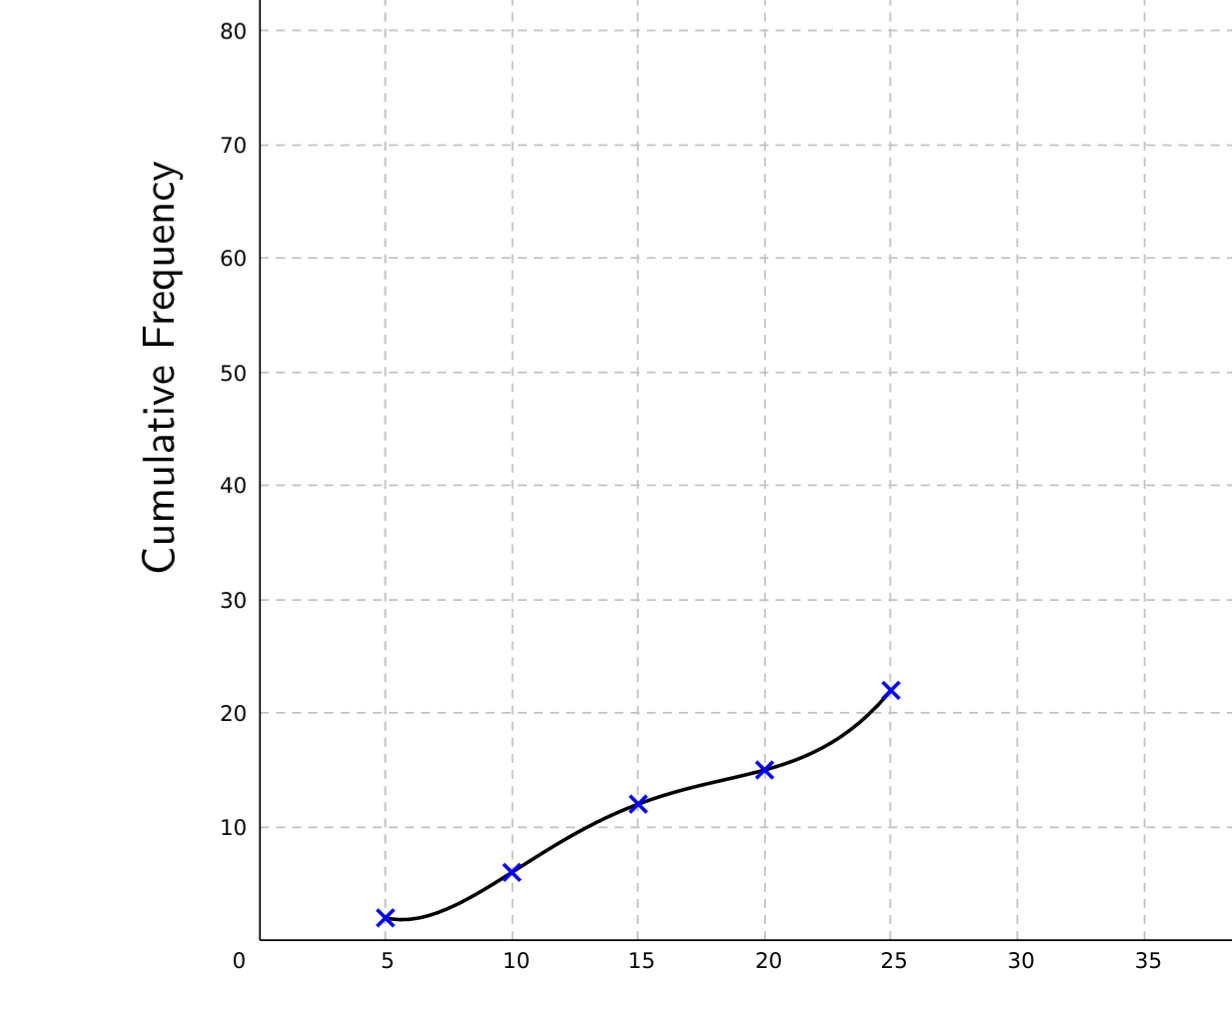
\includegraphics[scale=1.0]{cumulative-frequency-graph}
	\centering
	\caption{Example cumulative frequency graph. Note the curve should extend to 0}
\end{figure}

Estimating percentiles can be done by working out what the relevant percentile data point would be, for example the median would here be the 11th data point, and then seeing where curve is on the $y$-axis for 11 on the $x$-axis.

\subsubsection{Histograms}
Histograms are useful because they can be used on grouped data with unequal class widths. They are plotted similarly to bar charts (although with bars touching) with the data on the $x$-axis and frequency density on the $y$-axis. Frequency density is equal to frequency divided by class width, and this means that the area of a bar is equal to the frequency of the interval. By working out the area between any two points on the $x$-axis, it is possible to estimate the amount of data points between those two values.

\subsubsection{Comparing data}
Comparing data involves commenting either on measures of location, or on measures of spread. Sometimes, data will contain extreme values, which makes certain comparisions (like the median and interquartile range), better than others (for example the mean and range respectively).

	\section{Correlation}
\subsection{Bivariate data}
Bivariate data is data which maps one variable to another. An example might be visibility vs weather humidity. Correlation describes the nature of the linear relationship between these two variables.

Correlation can be strong or weak depending on how exactly the pattern is followed, and can be positive (one variable increases with the other), or negative (one variable decreases with the other). Data can also have no correlation.

\subsection{Linear regression}
Linear regression is used to accurately draw a line of best fit through the data. One way of doing this is using the least squares regression line, which minimises the value of the sum of the squares of the vertical distances of points away from the line.

The form of the linear regression line for $y$ on $x$ is $y=a+bx$, and can be found with a calculator. The coefficient $b$ tells whether the data is positively or negatively correlated, and how steep the line will be.

\subsection{Common issues with using regressions to make observations}
\subsubsection{Correlation $\ne$ causation}
If there is no proven causal link, then a causation is not enough to say that one metric affects the other. This can also be thought of as only being able to use the regression line to make predictions for values of the dependent variable rather than of the independent variable.

\subsubsection{Extrapolation vs interpolation}
Extrapolation is using trends in your data to predict things outside of the range, and is much less reliable than interpolation, which is the same but predicts things which are inside the range of the data.


	% \section{Algebraic methods}
\subsection{Proof by contradiction}
To prove by contradiction, the first step is to assume the negation of the statement. This negation statement is then used to arrive at a contradiction (statement we already know is untrue).
\subsubsection{Proof that $\sqrt{2}$ is irrational}
This proof is examinable.

First assume negation that $\sqrt{2}$ is rational, and can be written as a fraction $\frac{a}{b}$ in its simplest form ($a$ and $b$ have no common factors).

\begin{IEEEeqnarray}{rCl'r}
	\sqrt{2} & = & \frac{a}{b} & a, b \in \mathbb{Z}
	\nonumber\\
	2 & = & \frac{a^2}{b^2}
	\nonumber\\
	2b^2 & = & a^2
	\nonumber
\end{IEEEeqnarray}
This implies that $a^2$ is even, and so that $a$ is even. At this point we can let $a=2c$, $c \in \mathbb{Z}$

\begin{IEEEeqnarray}{rCl'r}
	2b^2 & = & (2c)^2
	\nonumber\\
	2b^2 & = & 4c^2
	\nonumber\\
	b^2 & = 2c^2
	\nonumber
\end{IEEEeqnarray}

This implies that $b^2$ is even, and so that $b$ is even.

This is a contradiction as $\frac{a}{b}$ is in fact not in its simplest form. Hence, $\sqrt{2}$ is irrational.

\subsubsection{Proof that there are infinitely many prime numberes}
This proof is examinable.

Assume negation that there is a finite list of primes, and let $P_1, P_2, P_3 \ldots P_n$ be this list.

Let $X=P_1 \times P_2 \times P_3 \ldots \times P_n$

$X>P_i$ for any $i$, so $X$ cannot be prime as it is not in the list.

Dividing $X$ by $P_i$ for any $i$ leaves remainder $1$, so $X$ cannot be product of primes.

So, $X$ is neither a prime or product of primes. This is a contradiction.

Hence, there are infinitely many prime numbers.

\subsection{Partial fractions}
A single fraction with two distinct linear factors in the denominator can be split into two partial fractions with linear denominators. To do this, first define variables as the numerators of these partial fractions, and then form an identity with the partial fractions. Next, multiply by the denominator of the full fraction, to set the numerators equal. Next values of $x$ can be substituted into the identity to eliminate the unknown partial fraction numerators.

\begin{IEEEeqnarray}{rCl}
	\frac{6x-2}{(x-3) (x+1)} & \equiv & \frac{A}{x-3}+\frac{B}{x+1}
	\nonumber\\
	6x-2 & \equiv & A(x+1) + B(x-3)
	\nonumber\\
	\text{When $x=-1$:}
	\nonumber\\
	6(-1)-2 & = & 0 + B((-1)-3)
	\nonumber\\
	-8 & = & -4B
	\nonumber\\
	B & = & 2
	\nonumber\\
	\text{When $x=3$:}
	\nonumber\\
	6(3)-2 & = & A((3)+1) + 0
	\nonumber\\
	16 & = & 4A
	\nonumber\\
	A & = & 4
	\nonumber\\
	\frac{6x-2}{(x-3) (x+1)} & \equiv & \frac{4}{x-3}+\frac{2}{x+1}
\end{IEEEeqnarray}

\subsubsection{When the denominator has a repeated factor}
If the denominator has a repeated factor, then one of the partial fractions will need to have that factor squared as a denominator so that it's possible to follow these steps without eliminating all of the variables. So $\frac{11x^2+14x+5}{(x+1)^2(2x+1)}$ would be split into $\frac{A}{x+1} + \frac{B}{(x+1)^2} + \frac{C}{2x+1}$.

\subsection{Improper algebraic fractions}
Improper algebraic fractions are defined as algebraic fractions with numerators which are polynomials of the same or a higher degree as their denominator.

To get rid of an improper algebraic fraction, two methods can be used.
\subsubsection{Fixing improper algebraic fractions with polynomial long division}
Polynomial long division can be used to fix algebraic fractions. Working out the remainder of the fraction means that it can be rewritten into just having the remainder over the denominator: if dividing $x^2+5x+8$ by $x-2$ give $x+7$ remainder $22$, then $\frac{x^2+5x+8}{x-2}=x+7+\frac{22}{x-2}$.

\subsubsection{Fixing improper algebraic fractions by forcing the denominator into the numerator}
By forcing the denominator into the numerator and subtracting other terms until the fractions are equal, it's possible to reduce the degree of the numerator polynomial until it's lower than the denominator.

This works by multiplying the denominator by something that will make the largest exponent in the numerator, and then separating the fraction and cancelling the denominators.
\begin{IEEEeqnarray}{rCl}
	\frac{x^2+5x+8}{x-2} & = & \frac{x(x-2)+7x+8}{x-2}
	\nonumber\\
	& = & x + \frac{7x+8}{x-2}
	\nonumber\\
	& = & x + \frac{7(x-2)-22}{x-2}
	\nonumber\\
	& = & x + 7 + \frac{22}{x-2}
\end{IEEEeqnarray}

\end{document}
